\section{Problema 1}

\subsection{Enunciado}
El enunciado nos plantea una situación en donde tenemos un edificio con n pisos y personas en cada piso que quiere ir a planta baja. Para poder hacerlo, el edificio provee un 
ascensor que deberá buscar a las personas para poder bajarlas. 
Este ascensor posee energía y capacidad limitada que no le permite recorrer siempre todos los pisos y levantar todas las personas, por lo tanto queremos maximizar la cantidad
de personas a descender del edificio dado la cantidad de personas por piso, su energía y la capacidad.

\subsection{Soluci\'on}
La solución planteada utiliza Programación Dinámica a través de decisiones. Es decir, planteamos el problema de forma tal que en vez de maximizar la cantidad de personas que 
pueden descender, encontramos el máximo valor posible que va a estar ubicado entre cero y la cantidad de personas total en el edificio.\\
A continuación se explicará cómo se resolvió el problema:\\
Primero obtenemos la cantidad total de personas recorriendo el edificio dado, y buscaremos ese dicho máximo valor.
Para ello, utilizaremos la conocida búsqueda binaria en la cantidad de personas en el edificio, hasta encontrar el valor tal que el siguiente no sea posible levantarlo y sin embargo el número que estoy evaluando si.
Por lo tanto lo único que resta, es ver si se puede levantar esa cantidad de personas dada la capacidad del ascensor, su energía y un edificio. \\
Para poder levantar esas personas buscaremos el piso mínimo al que necesitamos ir para poder levantar la cantidad de personas requeridas$^*$. Recorreremos el edificio desde ese piso mínimo hacia abajo, en caso de
ser posible llegar hasta él y poder volver a descender, levantando la máxima cantidad de personas de cada piso en el camino hasta llenar la capacidad. Una vez completada, descenderemos a los pasajeros y volveremos a repetir el proceso
para el mismo piso en caso de que haya quedado gente, o el siguiente en caso de haberlo vaciado o no poder llegar por poca energía, hasta que levantemos la cantidad requerida (caso que devolveremos que se puede) o hasta que nos quedemos sin energía (caso que devolveremos que no se puede). Tener en cuenta que el piso elegido como mínimo puede contener más cantidad de gente que la requerida por lo tanto puede pasar que no levantemos gente y que sin embargo, descendamos la cantidad requeridad personas.\\
Para la demostración de la resolución, explicaremos por qué el piso elegido previamente es el correcto, y por qué la estrategia de levantar de arriba hacia abajo es verdadera.
Este piso mínimo es la mejor opción ya que si subimos más pisos estaríamos utilizando energía para levantar la misma cantidad de gente que podríamos encontrar en los pisos
inferiores, y no se puede ir más abajo porque si no, tenemos la cantidad de gente necesaria para poder levantar el valor pedido.\\
Definimos el mundo de las estrategias, como el conjunto de estrategias posibles y definimos estrategia como el método por el que se levanta gente. Cómo no nos interesa
la energía utilizada, ya que solo queremos ver si puede levantar la cantidad de personas mencionada, y no la optimalidad de energía, una estrategia estará conformada por el
conjunto de personas que levanta en cada piso. De este mundo de estrategias, tomaremos solo aquellas que su piso más alto en el cual levantan personas es el nuestro, y que
levanten la misma cantidad que nosotros. Este conjunto es distinto de vacío ya que es un conjunto acotado de personas y pisos, por lo tanto se van a poder levantar a partir de
cierta energía dada. Ahora queremos ver que nuestra estrategia se encuentra en este conjunto. Para ello, tomaremos una de esas estrategias E y veremos que se puede permutar de tal
forma que consigamos nuestra estrategia. Esta permutación se debe a que si la estrategia E 


\small {\textbf{*} Para ubicar este piso mínimo recorreremos el edificio desde abajo contando la cantida de personas en los pisos, hasta que el valor sea mayor o igual al requerido.}




\subsection{Pseudoc\'odigo}
\begin{codebox}
\Procname{$\proc{resolver}$ (\textbf{in} $capacidad$, \textbf{in} $energia$, \textbf{in} $pisos$)}{maximaCantidad}{Int}
\li		totalPersonas = SumaTotalPersonas(pisos);
\li		return BusquedaBinariaPersonas(0,totalPersonas, totalPersonas,energia,capacidad,pisos);
\end{codebox}

\begin{codebox}
\Procname{$\proc{SumaTotalPersonas}$ (\textbf{in} $pisos$)}{acum}{Int}
\li		\textbf{Para} cada piso p \Do
\li			acum = acum + genteEnPiso(p) \End
\end{codebox}

\begin{codebox}
\Procname{$\proc{BusquedaBinariaPersonas}$ (\textbf{in} $desde$, \textbf{in} $hasta$, \textbf{in} $total$,\textbf{in} $energia$, \textbf{in} $capacidad$, \textbf{in} $pisos$)}{acum}{Int}
\li		medio = (desde + hasta)/2;
\li		puedo = sePuedeLevantar(energia, capacidad, pisos, medio);
\li 		\textbf{Si} puedo \Do
\li				\textbf{Si} no se puede levantar el siguiente terminé
\li 				\textbf{Si no} busquedaBinariaPersonas en la siguiente mitad \End
\li 		\textbf{Si no} busquedaBinariaPersonas en la primera mitad
\end{codebox}

\begin{codebox}
\Procname{$\proc{sePuedeLevantar}$ (\textbf{in} $energia$, \textbf{in} $capacidad$, \textbf{in} $pisos$, \textbf{in} $personasABuscar$)}{sePuede}{Boolean}
\li 		\textbf{Para} cada piso empezando desde el piso minimo \Do
\li			\textbf{Si} tengoEnergiaParaLlegar y Hay Gente \Do
\li				\textbf{Si} el piso tiene mas gente que mi capacidad \Do
\li					sumoLoQueLevante
\li					veoSiPuedoVolverAEstePiso \End
\li				\textbf{Si no} \Do
\li					sumoLoQueLevante
\li					mientrasBajoSumoGenteParandoEnLosPisosQueHayGente \End \End
\li			\textbf{Si no} \Do
\li				AnotoLasQueNoLevanté \End \End
\li		return (cuantoLevante >= personasABuscar)
\end{codebox}


\subsection{Analisís de complejidad}	
Para averiguar cuanta gente hay en todo el edificio tenemos que recorrer todo el vector 'pisos' e ir sumando la cantidad de gente en cada piso. Eso nos cuesto O(n) donde n es la cantidad de pisos. Luego hacemos una búsqueda binaria sobre la cantidad total de gente que mediante la función sePuedeLevantar busca el máximo de gente que es posible cargar. La complejidad de la búsqueda binaria es de O(log cantGente) (esto es sabido, porque ya lo vimos en algoritmos y estructura de datos 2) y la complejidad de la función sePuedeLevantar en el peor caso (sería cuando tiene que irse hasta el último piso para poder levantar la cantidad de gente solicitada y tiene energía suficiente para levantarlos a todos) es de: \\
	O( $\sum\limits_{i=0}^{n} { ( \lceil (pisos[i]/capacidad) \rceil  + i}$ ) ) \\
Esto es porque por cada piso al que voy tengo que ir tantas veces tal que levante el total de gente de ese piso (eso es $\lceil$pisos[i]/capacidad$\rceil$) y luego en caso que me haya sobrado espacio voy recorriendo todos los pisos inferiores para llenar la capacidad restante.
Finalmente la complejidad total del ejercicio nos queda:\\
O( n + Log(g) * $\sum\limits_{i=0}^{n} { ( \lceil (pisos[i]/capacidad) \rceil  + i ) }$ ) \\
Donde n es la cantidad total de pisos y g la cantidad total de gente en todo el edificio.

\subsection{Tests y Gráficos}
Con respecto a los tests realizados, los mismos no se hicieron en cuanto a la complejidad (ya que al utilizar estructuras primitivas de java, podemos asegurar que la complejidad de cada una de sus operaciones es la que aparece en la documentación de ellas y por tanto, es la que detallamos en el apartado anterior), sino en cuanto a la cantidad de ciclos que realiza cada solución (más precisamente, la creación del árbol generador mínimo) para distintas instancias, de acuerdo a la cantidad de vértices (localidades) y aristas (enlaces) que posee cada una.
Como podemos apreciar en los siguientes gráficos, la cantidad de ciclos, para grafos en donde la cantidad de aristas es la misma, es directamente proporcional a la cantidad de vértices que contenga el mismo (figura 1). Es cierto que en algunos casos ésto no se cumple pero, en el caso promedio, a más cantidad de vértices, con igual cantidad de aristas, más ciclos tendrá que hacer nuestro algoritmo para encontrar el AGM válido. Los casos extremos serían aquellos en donde las aristas se insertan ordenados de la misma forma que los leerá nuestro algoritmo, donde la cantidad de ciclos se corresponde con la cantidad de vértices. Por el contrario, el peor caso se da cuando hay muchas aristas de 2 vértices que ya fueron visitados, de menor peso de aquellas que contengan 1 vértice visitado y otro sin visitar. De ésta forma, el algoritmo hará tantos ciclos como aristas tenga el vértice para, recién en la último, procesar el vértice y agregarlo al AGM.
\begin {center}
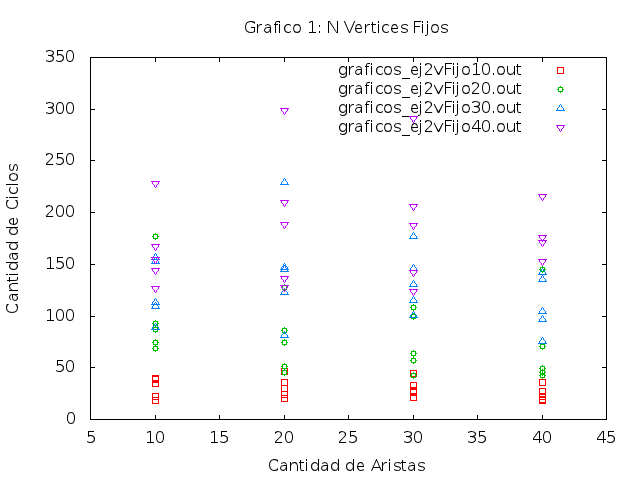
\includegraphics[width=8cm]{./graficos/grafico_vfijo.png}
% grafico.eps: 0x0 pixel, 300dpi, 0.00x0.00 cm, bb=50 50 410 302
\end {center} 
Por otro lado, y con respecto a la figura 2, donde la cantidad de aristas está fijo, vemos que la cantidad de ciclos que se llevan a cabo es netamente aleatorio, ya que, de acuerdo a cómo estén distribuidas las distintas aristas y sus pesos, es posible crear el AGM en n pasos, siendo n la cantida de vértices, o bien, en n x e(n), siendo e(n) la cantidad de aristas de n. El primer caso se daría sólo cuando el grafo que analizamos posee aristas minimas sin descubrir en todos los pasos, mientras que el peor caso, que sería el de recorrer todas las aristas del vértice, es el mismo que analizamos en el párrafo anterior.
\begin {center}
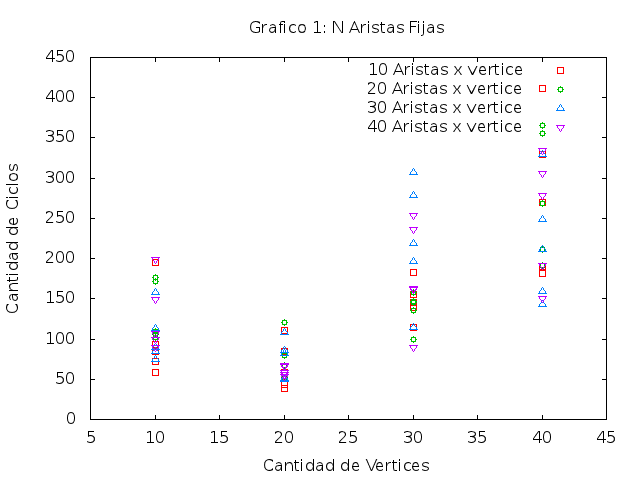
\includegraphics[width=8cm]{./graficos/grafico_efijo.png}
% grafico.eps: 0x0 pixel, 300dpi, 0.00x0.00 cm, bb=50 50 410 302
\end {center} 


\subsection{Conclusiones}
El problema nos mostró que podía ser encarado de distintas maneras dentro de la métodología de programación dinámica. Al principio habíamos utilizado una idea parecida a la de SubSetSum con memorization pero no podíamos hacer funcionar el algoritmo. Sin embargo, encaramos el problema a través de decisiones lo que nos ayudó a entender el principio de ptimalidad.
